\chapter{Alternative Methods}
\label{cha:alternative_methods}

The performance of the CNN is compared to alternative methods to put the results into perspective.
The alternative methods are the Support Vector Machine (SVM), the Logistic Regression (LR), and the k-Nearest Neighbors (kNN) algorithm that are implemented in the scikit-learn library \cite{scikit-learn}.
The models are not optimized in this work and the default hyperparameters are used.
They use the first- and second-order features as input.
First-order features are mean, variance, skewness, kurtosis, and entropy.
Second-order features are contrast, energy, angular second moment (ASM), entropy, homogeneity, dissimilarity, correlation, and coarseness.
The features are extracted from the MRI images. %and are used as input for the binary classification models.
To explore the data, the features are visualized in a comparison between benign and malignant brain tumours in Figure \ref{fig:benign_malignant_comparison}.
\begin{figure}[H]
    \centering
    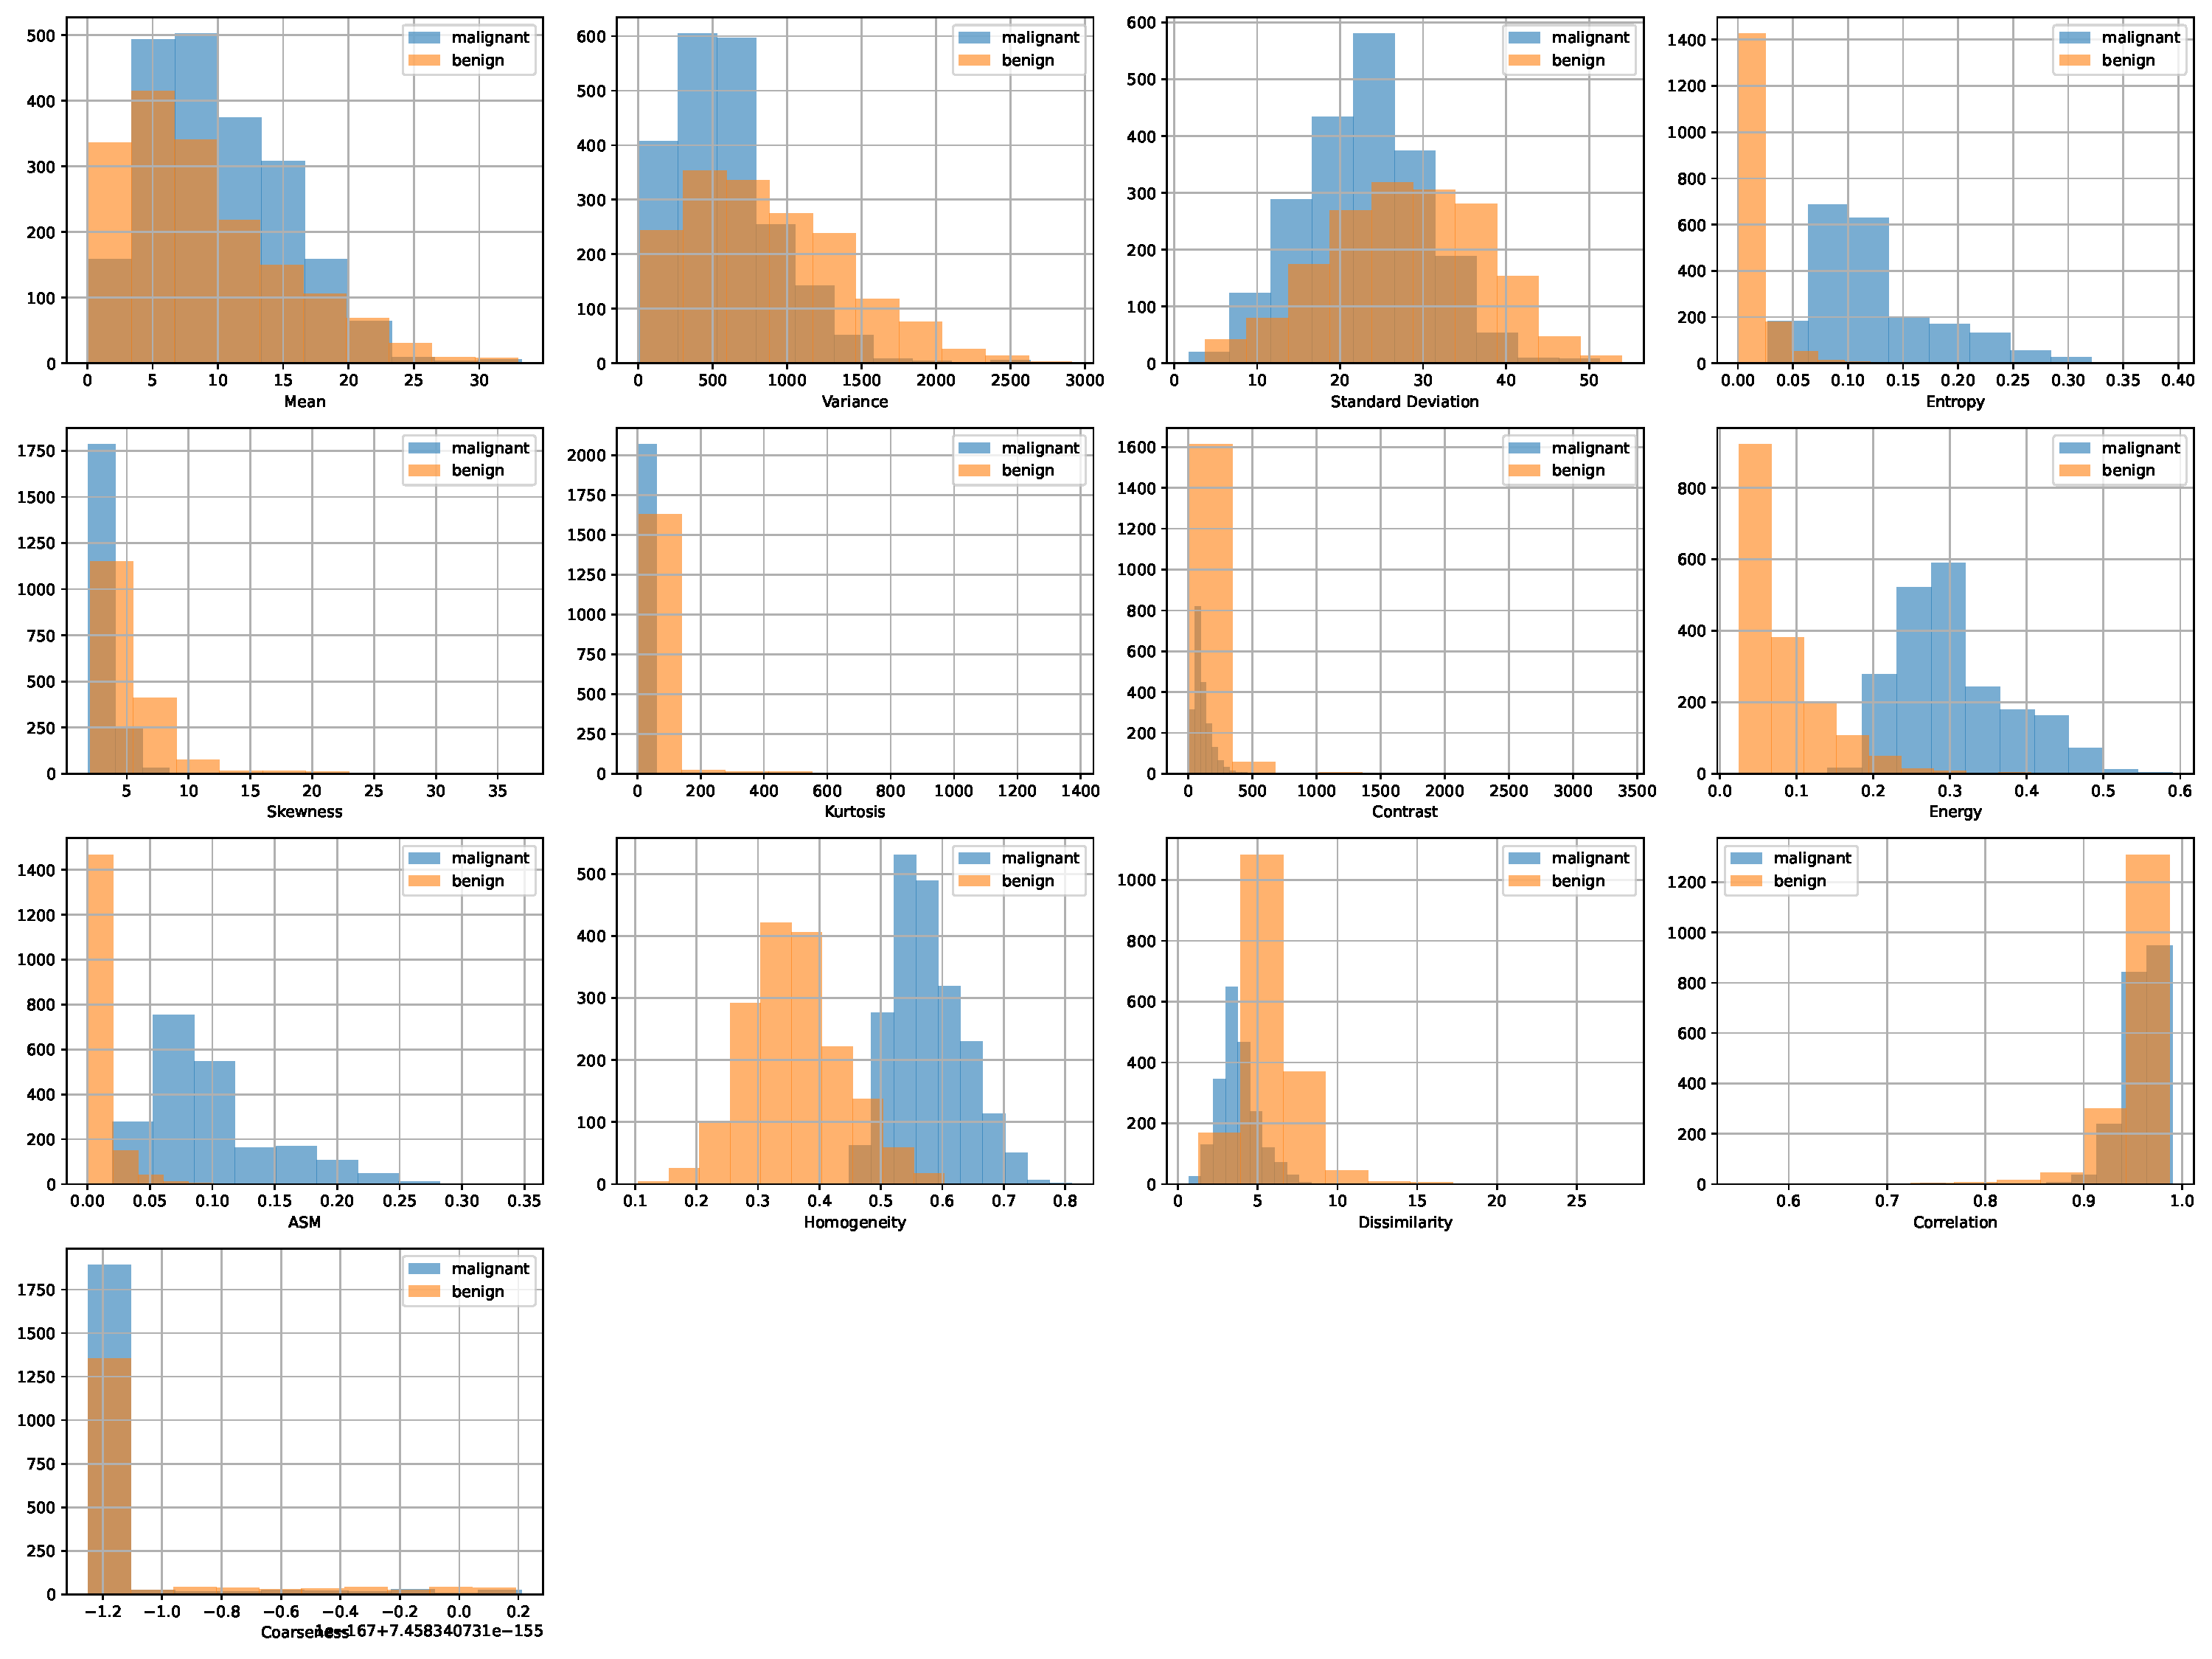
\includegraphics[width=.8\textwidth]{plots/benign_malignant_comparison.pdf}
    \caption{Comparison between benign and malignant brain tumours for the first- and second-order features.}
    \label{fig:benign_malignant_comparison}
\end{figure}
It can be seen that the entropy, the energy, the ASM and the homogeneity are the most promising features to distinguish between benign and malignant brain tumours.
Other features such as the dissimilarity show not a high difference between the two classes.
With the difference in the first three features being so distinctive, however, it can be concluded that they are well suited for the classification task.
The alternative algorithms should be able to distinguish between benign and malignant brain tumours very well, based on these features.
This behaviour can also be seen in the correlation between the features that are calculated and discussed in section \ref{sec:DataExploration}.
% From this comparison, it can be concluded that the features are well suited for the classification task and that the models should be able to distinguish between benign and malignant brain tumours very well.

Before the models are built, the data is split into a training and a test set with a ratio of 80:20 and scaled using the standard scaler from scikit-learn.
The models calculate a fit on the training data and predict the labels on the test data.

\section{Comparison to the CNN}
\label{sec:comparison}

The performance of the models is again evaluated on the same metrics as the CNNs before.
The results are shown in Table \ref{tab:comparisonTable}.
All of the alternative methods produce very good results and they outperform the initial CNN.
The SVM and the LR have the best recall of 96.17\%, which is slightly better than the final CNN with a recall of 95.19\%.
Both of the models outperform every other model on the other metrics as well, except for the precision of the kNN, which is 100\%.
The final CNN, however, can outperform the kNN in the recall and its precision is even better than the LR.
The metrics show that the alternative methods are very well suited for the classification task and can outperform the CNNs.
\begin{table}[H]
    \centering
    \caption{Comparison of the alternative methods to the initial and the final CNN, sorted by the recall.}
    \label{tab:comparisonTable}
    \begin{tabular}{c | c c c c c c c}
        \toprule
        model & recall & accuracy & precision & f1-score & $R^2$-score & Mean Squared Error \\ 
        \midrule
        SVM & 0.9617 & 0.9801 & 0.9939 & 0.9775 & 0.9195 & 0.0199 \\
        LR & 0.9617 & 0.9788 & 0.9909 & 0.9760 & 0.9141 & 0.02124 \\
        final CNN & 0.9519 & 0.9694 & 0.9925 & 0.9718 & 0.8763 & 0.0306 \\ 
        kNN & 0.9469 & 0.9761 & 1.0 & 0.9727 & 0.9034 & 0.0239 \\
        initial CNN & 0.8726 & 0.9229 & 0.9864 & 0.9260 & 0.6880 & 0.0771 \\
        \bottomrule
    \end{tabular}
\end{table}


% \begin{figure}[H]
%     \centering
%     \begin{subfigure}[B]{.45\textwidth}   % 1st subfigure
%         \centering
%         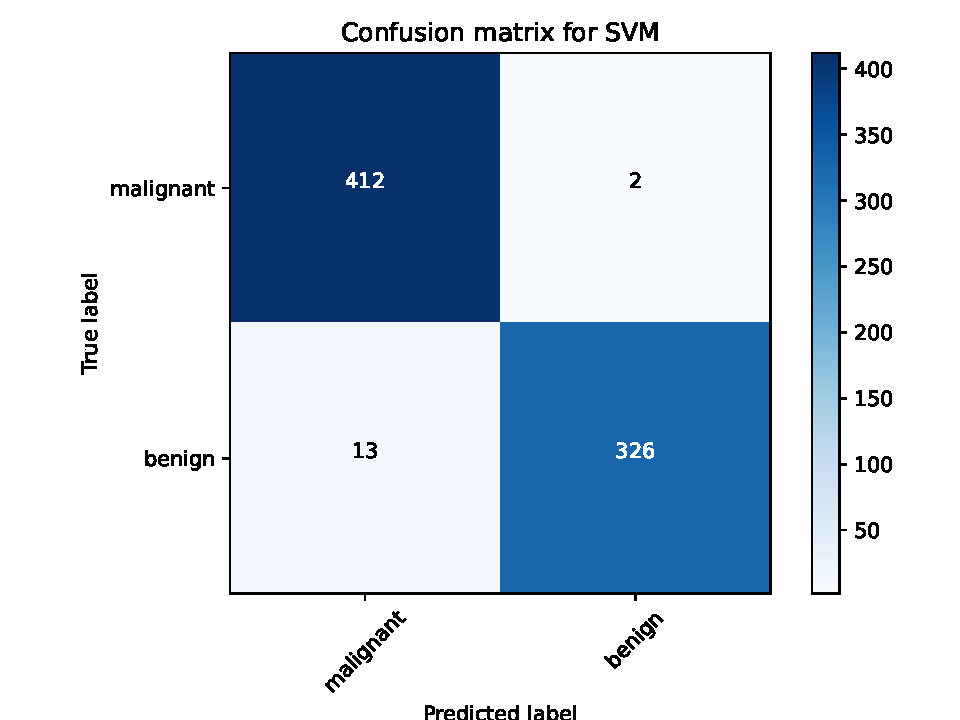
\includegraphics[width=\linewidth]{plots/confusion_matrix_SVM.pdf}
%         \caption{Confusion matrix of the SVM.}
%         \label{fig:confusion_matrix_SVM}
%     \end{subfigure}    
%     \begin{subfigure}[B]{.45\textwidth}   % 2nd subfigure
%         \centering
%         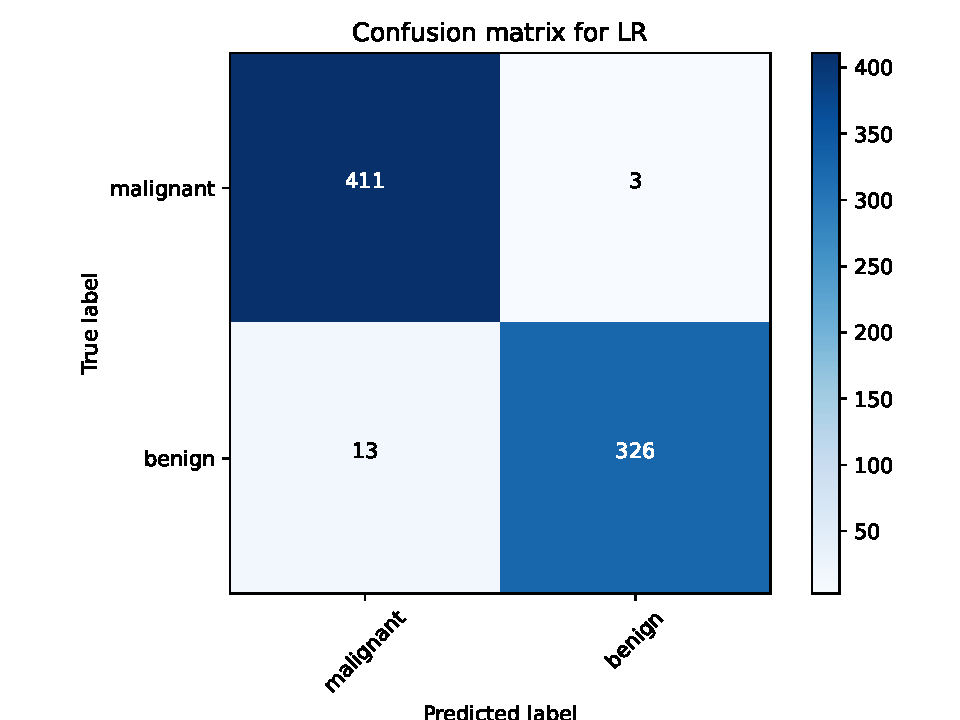
\includegraphics[width=\linewidth]{plots/confusion_matrix_LR.pdf}
%         \caption{Confusion matrix of the LR.}
%         \label{fig:confusion_matrix_LR}
%     \end{subfigure}
%     \begin{subfigure}[B]{.45\textwidth}   % 3rd subfigure
%         \centering
%         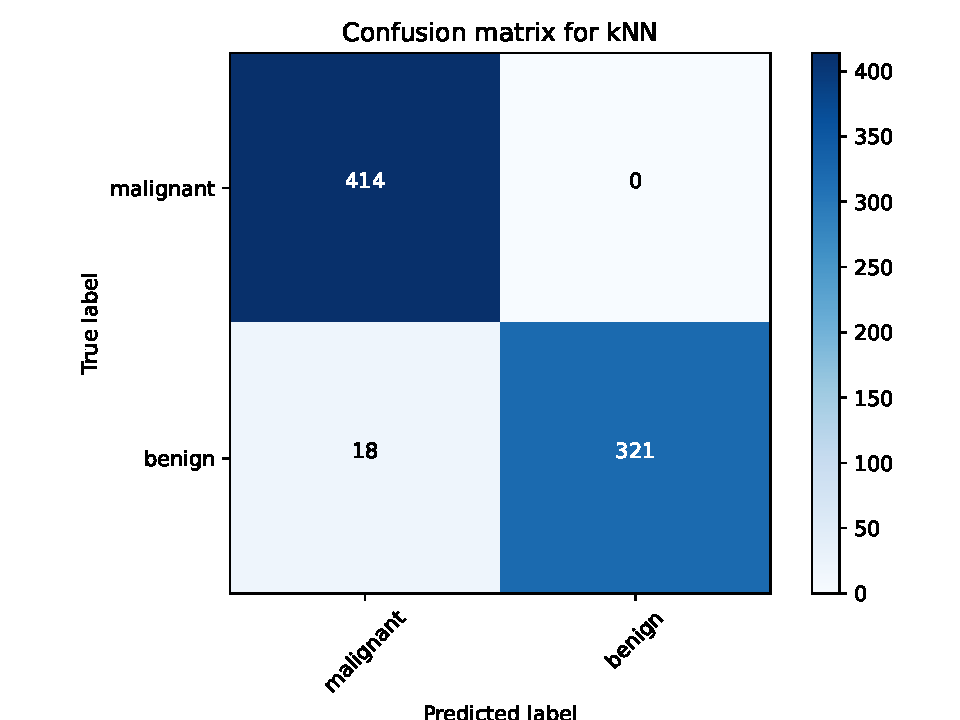
\includegraphics[width=\linewidth]{plots/confusion_matrix_kNN.pdf}
%         \caption{Confusion matrix of the kNN.}
%         \label{fig:confusion_matrix_kNN}
%     \end{subfigure}
%     \caption{Confusion matrices of the alternative methods.}
%     \label{fig:confusion_matricesAlternativeMethods}
% \end{figure}